%*****************************************
\chapter{Data}\label{06:data}
%*****************************************
%TODO Status: pre-draft

\begin{wrapfigure}{r}{0.4\textwidth}
	\label{06:fig01} 
	\centering
	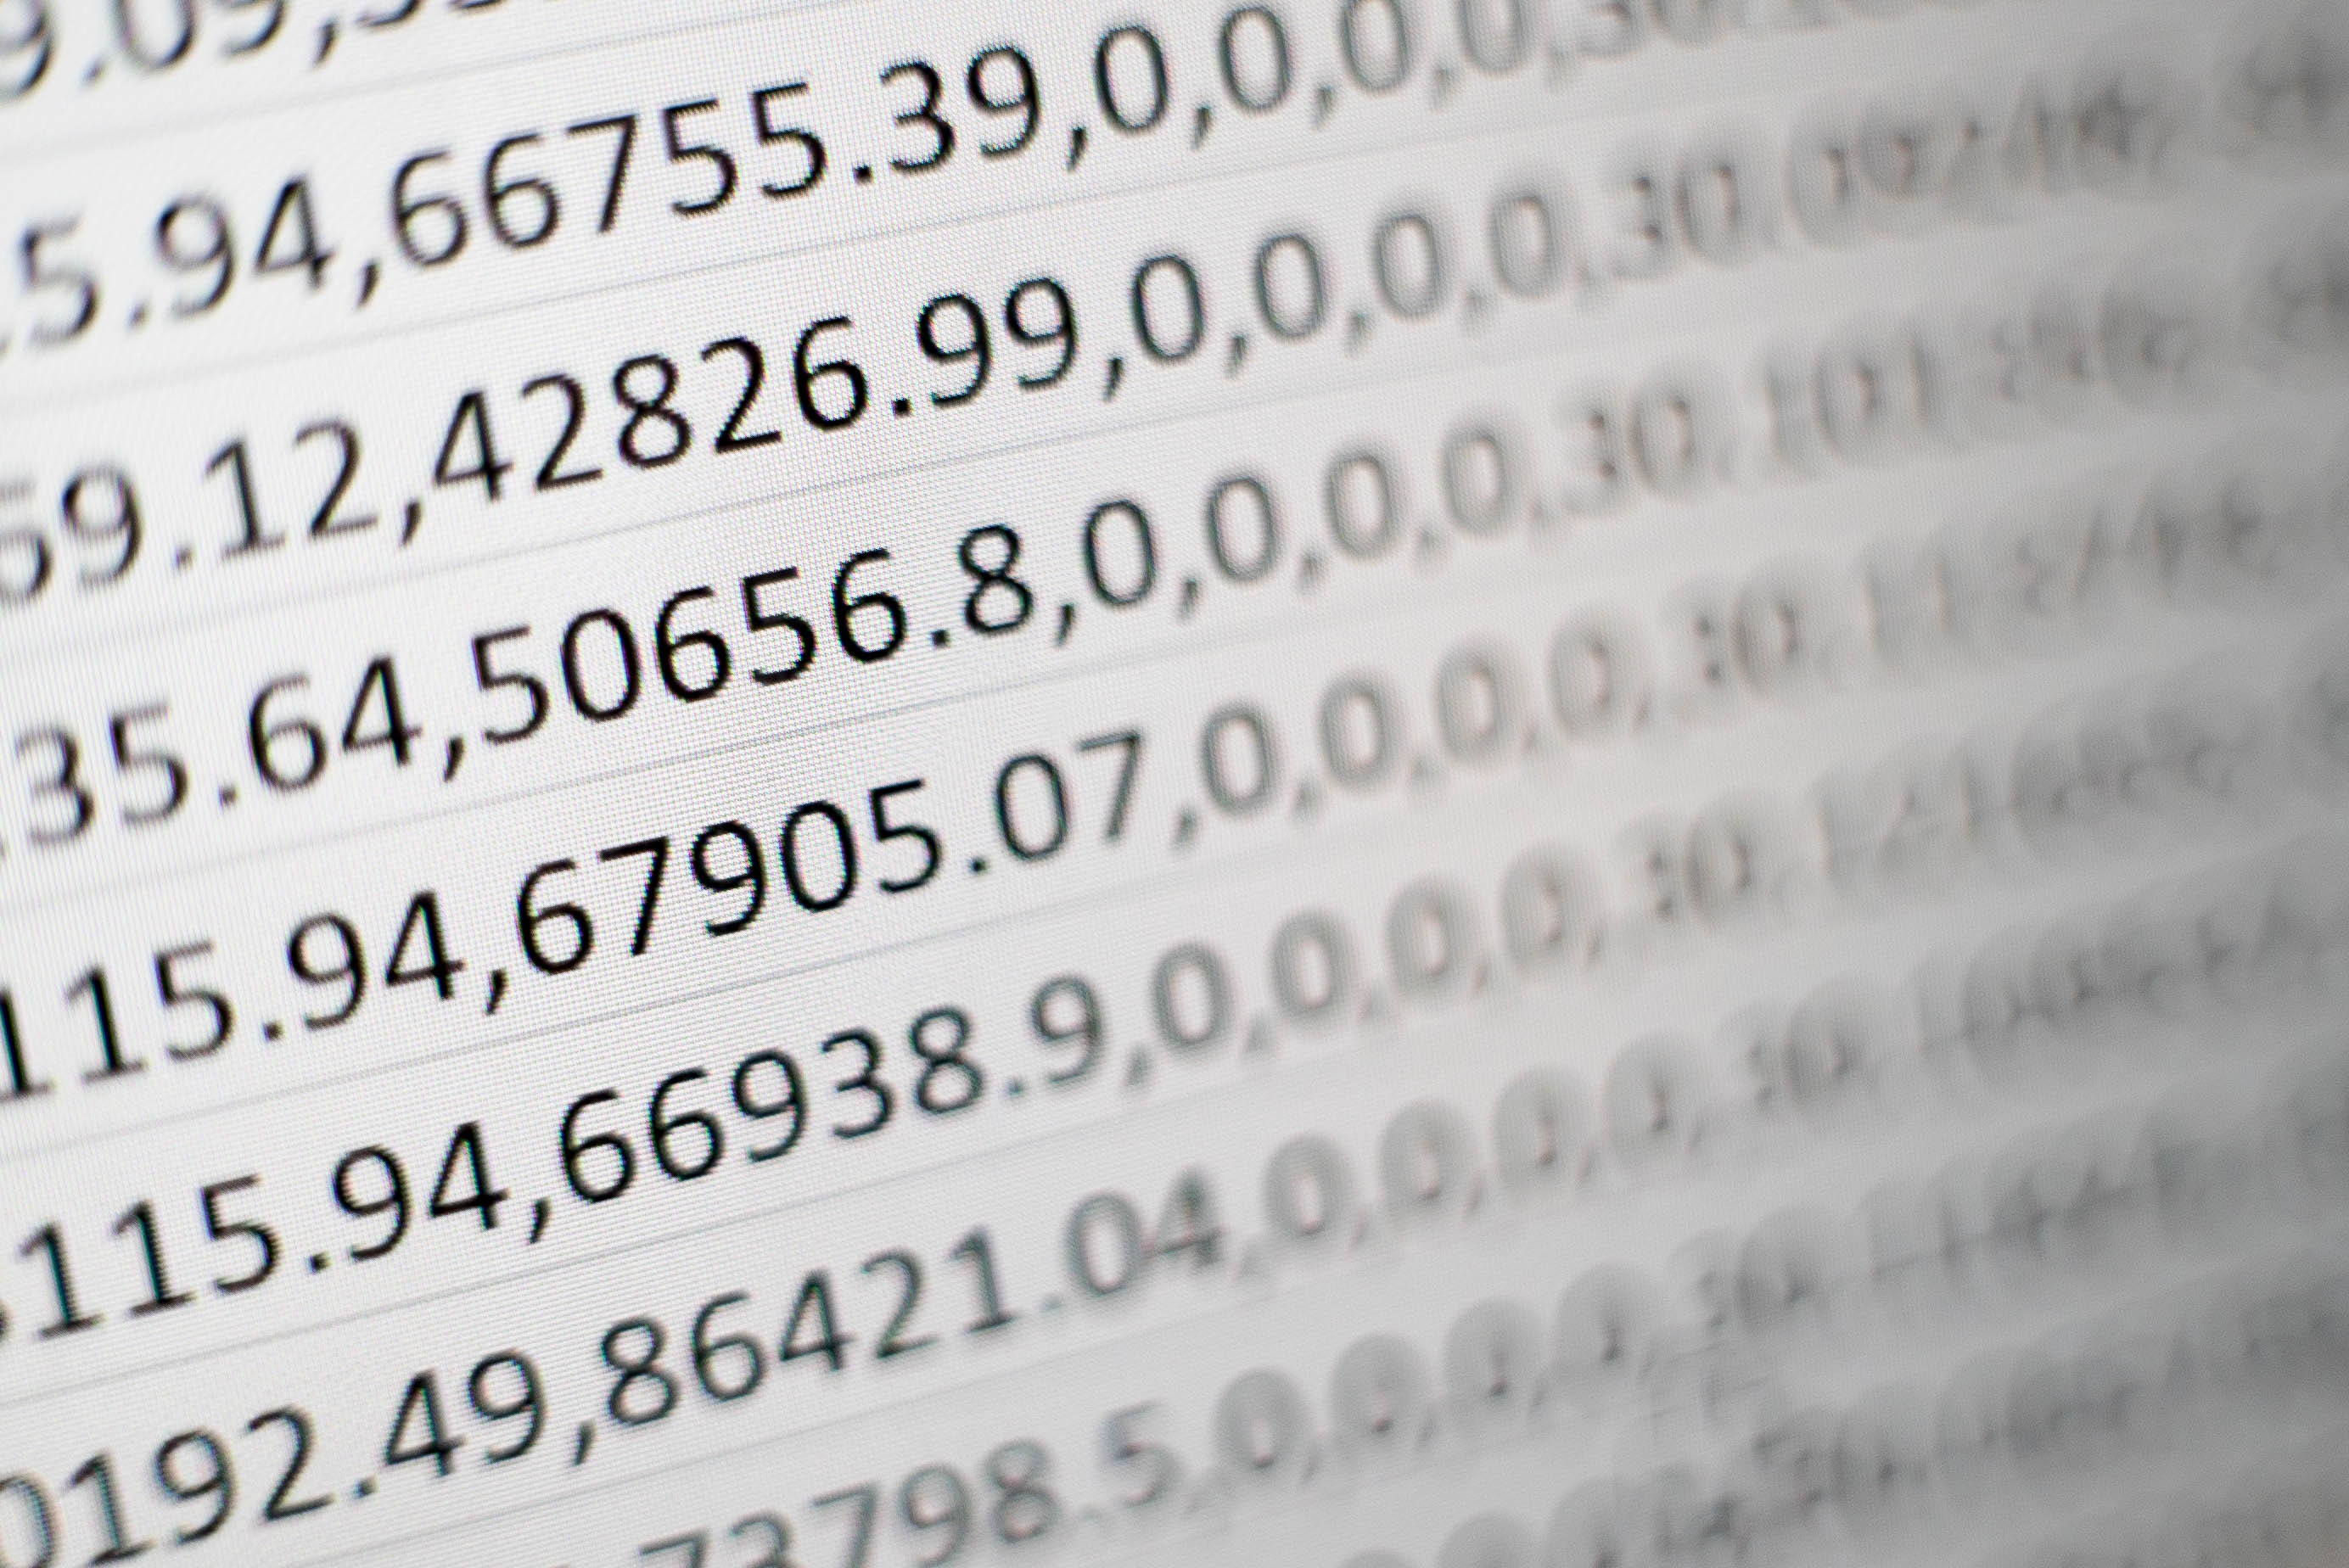
\includegraphics[width=0.4\textwidth]{gfx/06-data} 
\end{wrapfigure}
Data are\footnote{The word ``data'' is plural and is treated that way in this text even though modern usage seems to be trending toward a singular form.} a collection of facts about some topic. As examples, a ``customer loyalty'' program gathers data from customers on how often they shop, what they purchase on each trip, what time of day they typically shop, and all sorts of other data. When data are interpreted in some way they become information. The types of analyses that can be done with data are limited by the types of data involved. The purpose of this chapter is to introduce various concepts about data and show how they can be analyzed.\footnote{Photo by Mika Baumeister on Unsplash}

\subsection{Types of Data}

Psychologist Stanley Smith Stevens defined four generic types of data\cite{stevens1946theory}. 

\begin{itemize}
	
	\item \textbf{\Gls{qualitativedata}} groups observations into a limited number of categories; for example, type of pet (cat, dog, bird, etc.) or place of residence (Arizona, California, etc.). Because qualitative data do not have characteristics like means or standard deviations, they are analyzed using non-parametric tests, like Kruskal-Wallis H and Mann-Whitney U. Qualitative data can be further divided into two sub-types, nominal and ordinal.
	
	\begin{itemize}
		\item \textbf{\Gls{nominaldata}} are categories that do not overlap and have no meaningful order, they are merely labels for attributes. Examples of nominal data include occupations (custodial, accounting, sales, etc.) and blood type (A, B, AB, O). A special subcategory of nominal data is binary, or dichotomous, where there are only two possible responses, like ``yes'' and ``no''. Nominal data are sometimes stored in a database using numbers but they cannot be treated like numeric data. For example, binary data, like ``Do you rent or own your home?'' can be stored as ``1 = rent, 2 = own'' but the numbers in this case have no numeric significance and could be replaced by words like ``Rent'' and ``Own.''
		
		\item \textbf{\Gls{ordinaldata}} are categorical data but, unlike nominal, the categories imply some sort of order (which is why it is called ``ordinal'' data). One example of ordinal data is the ``star'' rating system for movies. It is clear that a five-star movie is somehow better than a four-star movie but there is no way to quantify the difference between those two categories. As another example, it is common for hospital staff members to ask patients to rate their pain level on a scale of one to ten. If a patient reports a pain level of ``seven'' but after some sort of treatment later reports a pain level of ``five'' then the pain has clearly decreased but it would be impossible to somehow quantify the exact difference in those two levels. Ordinal scales are most commonly used with Likert-type survey questions where the responses are selections like ``Strongly Agree'', ``Agree'', ``Neutral'', ``Disagree'', ``Strongly Disagree''. Ordinal data are also used when numeric data are grouped. For example, if a dataset included respondents' ages then those numbers could be grouped into categories like ``$ 20-29 $'' and ``$ 30-39 $.'' Those groups would typically be stored in the dataset as a single number so maybe ``$ 2 $'' would represent the ages ``$ 20-29 $,'' which would be ordinal data.
	\end{itemize}
	
	\item \textbf{\Gls{quantitativedata}} are numbers, typically counts or measures, like a person's age, a tree's height, or a truck's weight. Quantitative data are measured with scales that have equal divisions so the difference between any two values can be calculated. Quantitative data are discrete if they are represented by integers, like the count of words in a document, or continuous if they are represented by fractional numbers, like a person's height. Because quantitative data includes characteristics like means and standard deviations, they are analyzed using parametric tests, like T-tests and Analysis of Variance (ANOVA). Quantitative data can be further divided into two sub-types, interval and ratio.
	
	\begin{itemize}
		\item \textbf{\Gls{intervaldata}} use numbers to represent quantities where the distance between any two quantities can be calculated but there is no true zero point on the scale. One example is a temperature scale where the difference between $ 80 $\textdegree and $ 90 $\textdegree is the same as the difference between $ 60 $\textdegree and $ 70 $\textdegree. It is important to note that interval data do not include any sort of true zero point, thus zero degrees Celsius does not mean ``no temperature,'' and without a zero point it is not reasonable to make a statement like $ 20 $\textdegree is twice as hot as $ 10 $\textdegree.
		
		\item \textbf{\Gls{ratiodata}} use numbers to describe a specific measurable distance between two quantities; however, unlike interval data, ratio data have a true zero point. A good example of ratio data is the sales report for an automobile dealership. Because the data are a simple count of the number of automobiles sold it is possible to compare on month with another. Also, since the scale has a true zero point (it is possible to have zero sales) it is possible to state that one month had twice the sales of another.
	\end{itemize}
\end{itemize}

\section{Rating Scale}

When working with qualitative data, it is important for researchers to determine a rating scale, also called levels of measure, to record data gathered about any one attribute. For example, male-female-other, M-F-O, and $ 1 $-$ 2 $-$ 3 $ are three potential rating scales for the attribute \textit{gender}. A researcher could use any of these scales, or devise a completely different one, as long as the scale is used consistently throughout the entire research project. It is easy to imagine that many rating scales exist but the most common ones are \textit{binary}, \textit{Likert}, \textit{semantic differential}, and \textit{Guttman}. 

\begin{description}
	\item[Binary] Binary scales are nominal scales consisting of binary items that assume one of only two possible values, such as yes or no, true or false, and so on. For example, a typical binary scale for a ``political activism'' construct may consist of the six binary items shown in Table \ref{tab06.02}. Each item in this scale is a binary item, and the total number of ``yes'' indicated by a respondent (a value from $ 0 $ to $ 6 $) can be used as an overall measure of that person's political activism. Binary scales can also employ other values, such as male or female for gender, full-time or part-time for employment status, and so forth. If an employment status item is modified to allow for more than two possible values (e.g., unemployed, full-time, part-time, and retired), it is no longer binary, but still remains a nominal scaled item.
	
	\begin{table}[H]
		\centering
		\begin{tabularx}{0.95\linewidth}{p{0.70\linewidth}p{0.09\linewidth}p{0.09\linewidth}}
			\toprule
			\textbf{Question} & \textbf{Yes} & \textbf{No} \\
			\midrule
			Have you ever written a letter to a public official? & $ \bigcirc $ & $ \bigcirc $ \\ 
			Have you ever signed a political petition? & $ \bigcirc $ & $ \bigcirc $ \\ 
			Have you ever donated money to a political cause? & $ \bigcirc $ & $ \bigcirc $ \\ 
			Have you ever donated money to a candidate running for public office? & $ \bigcirc $ & $ \bigcirc $ \\ 
			Have your ever written a political letter to the editor of a newspaper?& $ \bigcirc $ & $ \bigcirc $ \\ 
			Have you ever persuaded someone to change his/her voting plans? & $ \bigcirc $ & $ \bigcirc $ \\ 
			\bottomrule
		\end{tabularx}
		\caption{Political activism binary scale}
		\label{tab06.02}
	\end{table}
	
	\item[Likert] Designed by Rensis Likert, this is a very popular rating scale for measuring ordinal data in business research. This scale includes Likert items that are simply-worded statements to which respondents can indicate their extent of agreement or disagreement on a five or seven-point scale ranging from ``strongly disagree'' to ``strongly agree.'' A typical example of a six-item Likert scale for the ``employment self-esteem'' construct is shown in table \ref{tab06.03}. Likert scales are summated scales, that is, the overall scale score may be a summation of the attribute values of each item as selected by a respondent.
	
	\begin{table}[H]
		\centering
		\begin{tabularx}{0.95\linewidth}{p{0.35\linewidth}p{0.10\linewidth}p{0.08\linewidth}p{0.07\linewidth}p{0.07\linewidth}p{0.08\linewidth}}
			\toprule
			{\footnotesize Statement} & {\footnotesize Strongly disagree} & {\footnotesize Disagree} & {\footnotesize Neutral} & {\footnotesize Agree} & {\footnotesize Strongly agree} \\
			\midrule
			{\footnotesize I feel good about my job} & $ \bigcirc $ & $ \bigcirc $ & $ \bigcirc $ & $ \bigcirc $ & $ \bigcirc $ \\
			{\footnotesize I get along well with others at work} & $ \bigcirc $ & $ \bigcirc $ & $ \bigcirc $ & $ \bigcirc $ & $ \bigcirc $ \\
			{\footnotesize I'm proud of my relationship with my supervisor} & $ \bigcirc $ & $ \bigcirc $ & $ \bigcirc $ & $ \bigcirc $ & $ \bigcirc $ \\
			{\footnotesize I feel like I'm making a contribution at work} & $ \bigcirc $ & $ \bigcirc $ & $ \bigcirc $ & $ \bigcirc $ & $ \bigcirc $ \\
			{\footnotesize I can tell that my coworkers respect me} & $ \bigcirc $ & $ \bigcirc $ & $ \bigcirc $ & $ \bigcirc $ & $ \bigcirc $ \\
			\bottomrule
		\end{tabularx}
		\caption{Likert scale for employee self-esteem}
		\label{tab06.03}
	\end{table}
	
	Likert items allow for more granularity (more finely tuned response) than binary items, including whether respondents are neutral to the statement. Three or nine values (often called ``anchors'') may also be used, but it is important to use an odd number of values to allow for a ``neutral'' (or ``neither agree nor disagree'') anchor. Some studies have used a ``forced choice approach'' to force respondents to agree or disagree with the Likert statement by dropping the neutral mid-point and using even number of values, but this is not a good strategy because some people may indeed be neutral to a given statement and the forced choice approach does not provide them the opportunity to record their neutral stance. A key characteristic of a Likert scale is that even though the statements vary in different items or indicators, the anchors (``strongly disagree'' to ``strongly agree'') remain the same. Likert scales are ordinal scales because the anchors are not necessarily equidistant, even though sometimes we treat them like interval scales.
	
	\item[Semantic Differential] This is a composite (multi-item) scale where respondents are asked to indicate their opinions or feelings toward a single statement using different pairs of adjectives framed as polar opposites. For instance, the construct ``attitude toward health insurance'' can be measured using three items shown in Table \ref{tab06.04}. As in the Likert scale, the overall scale score may be a summation of individual item scores. Notice that in Likert scales, the statement changes but the anchors remain the same across items. However, in semantic differential scales, the statement remains constant, while the anchors (adjective pairs) change across items. Semantic differential is believed to be an excellent technique for measuring people's attitude or feelings toward objects, events, or behaviors. 
	
	
	\begin{table}[H]
		\centering
		\begin{tabularx}{0.95\linewidth}{p{0.10\linewidth}p{0.10\linewidth}p{0.10\linewidth}p{0.10\linewidth}p{0.10\linewidth}p{0.10\linewidth}p{0.10\linewidth}}
			\toprule
			\multicolumn{7}{p{0.95\linewidth}}{How would you rate your opinion on health insurance?} \\	
			\midrule
			{} & {\footnotesize Very Much} & {\footnotesize Much} & {\footnotesize Neutral} & {\footnotesize Much} & {\footnotesize Very Much} & {} \\
			\midrule
			{\footnotesize Good} & $ \bigcirc $ & $ \bigcirc $ & $ \bigcirc $ & $ \bigcirc $ & $ \bigcirc $ & {\footnotesize Bad} \\
			{\footnotesize Useful} & $ \bigcirc $ & $ \bigcirc $ & $ \bigcirc $ & $ \bigcirc $ & $ \bigcirc $ & {\footnotesize Useless} \\
			{\footnotesize Caring} & $ \bigcirc $ & $ \bigcirc $ & $ \bigcirc $ & $ \bigcirc $ & $ \bigcirc $ & {\footnotesize Uncaring} \\
			\bottomrule
		\end{tabularx}
		\caption{Semantic differential scale}
		\label{tab06.04}
	\end{table}
	
	\item[Guttman] Designed by Louis Guttman, this composite scale uses a series of items arranged in increasing order of intensity of the construct of interest, from least intense to most intense. As an example, the construct ``attitude toward immigrants'' can be measured using five items shown in Table \ref{tab06.05}. Each item in the Guttman scale has a weight (not indicated above) which varies with the intensity of that item, and the weighted combination of each response is used as aggregate measure of an observation.
	
	\begin{table}[H]
		\centering
		\begin{tabularx}{0.95\linewidth}{p{0.70\linewidth}p{0.10\linewidth}p{0.10\linewidth}}
			\toprule
			\multicolumn{3}{p{0.95\linewidth}}{How will you rate your opinion on the following statements about immigrants?} \\	
			\midrule
			Do you mind immigrants being citizens of your country? & Yes & No \\
			Do you mind immigrants living in your own neighborhood? & Yes & No \\
			Would you mind living next door to an immigrant? & Yes & No \\
			Would you mind having an immigrant as your close friend? & Yes & No \\
			Would you mind if someone in your family married an immigrant? & Yes & No \\		
			\bottomrule
		\end{tabularx}
		\caption{Guttman scale}
		\label{tab06.05}
	\end{table}
	
\end{description}



\section{Properties of Data}

\subsection{About The Normal Distribution (Bell Curve)}

When the quantitative data gathered from some statistical project are plotted on a graph they often form a \gls{normaldistribution} (sometimes called a ``bell curve'' due to its shape). As an example, consider the Scholastic Aptitude Test (SAT) which is administered to more than $ 1.5 $ million high school students every year. Figure \ref{fig06.01} was created with fake data but illustrates the results expected of a typical SAT administration.

\begin{figure}[H]
	\centering
	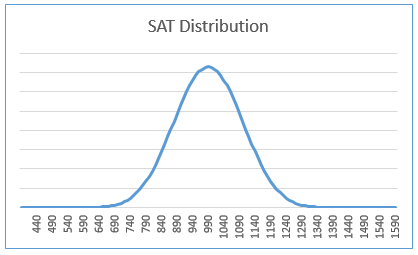
\includegraphics[width=\maxwidth{.95\linewidth}]{gfx/06-SATDistro}
	\caption{Normal Distribution}
	\label{fig06.01}
\end{figure}

SAT scores lie between $ 400 $ and $ 1600 $ as listed across the X-Axis and the number of students who earn each score is plotted. Since the most common score is $ 1000 $ that score is at the peak of the curve. Very few students scored above $ 1300 $ or below $ 650 $ and the curve is near the lower bound beyond those points. This illustrates a normal distribution where most scores are bunched near the center of the graph with only a few at either extreme.

The normal distribution is important because it permits researchers to use specific techniques to test a hypothesis about the sample. For example, perhaps a researcher hypothesized that the graduation rate at university ``A'' was higher than at university ``B'' because students' SAT scores were higher. Since SAT scores have a normal distribution, the researcher could use specific tests, like a t-test, to support or refute the hypothesis. However, if the data were not normally distributed then the researcher would need to use a different group of tests.

\subsection{Excess Kurtosis}
One way to mathematically describe a normal distribution is to calculate the length of the tails of a bell curve, and that is called its \gls{excesskurtosis}. For a normal distribution the excess kurtosis is $ 0.00 $, a positive excess kurtosis would indicate longer tails while a negative excess kurtosis would indicate shorter tails. Intuitively, many people believe the excess kurtosis represents the ``peaked-ness'' of the curve since longer tails would tend to lead to a more peaked graph; however, excess kurtosis is a measure of the data outliers, which would be only present in the tails of the graph; so excess kurtosis is not directly indicative of the the ``sharpness'' of the peak. It is difficult to categorically state that some level of excess kurtosis is good or bad. In some cases, data that form a graph with longer tails are desired but in other cases they would be a problem.

Following are three examples of excess kurtosis. Notice that as the excess kurtosis increases the tails become longer. 

\begin{figure}[H]
	\centering
	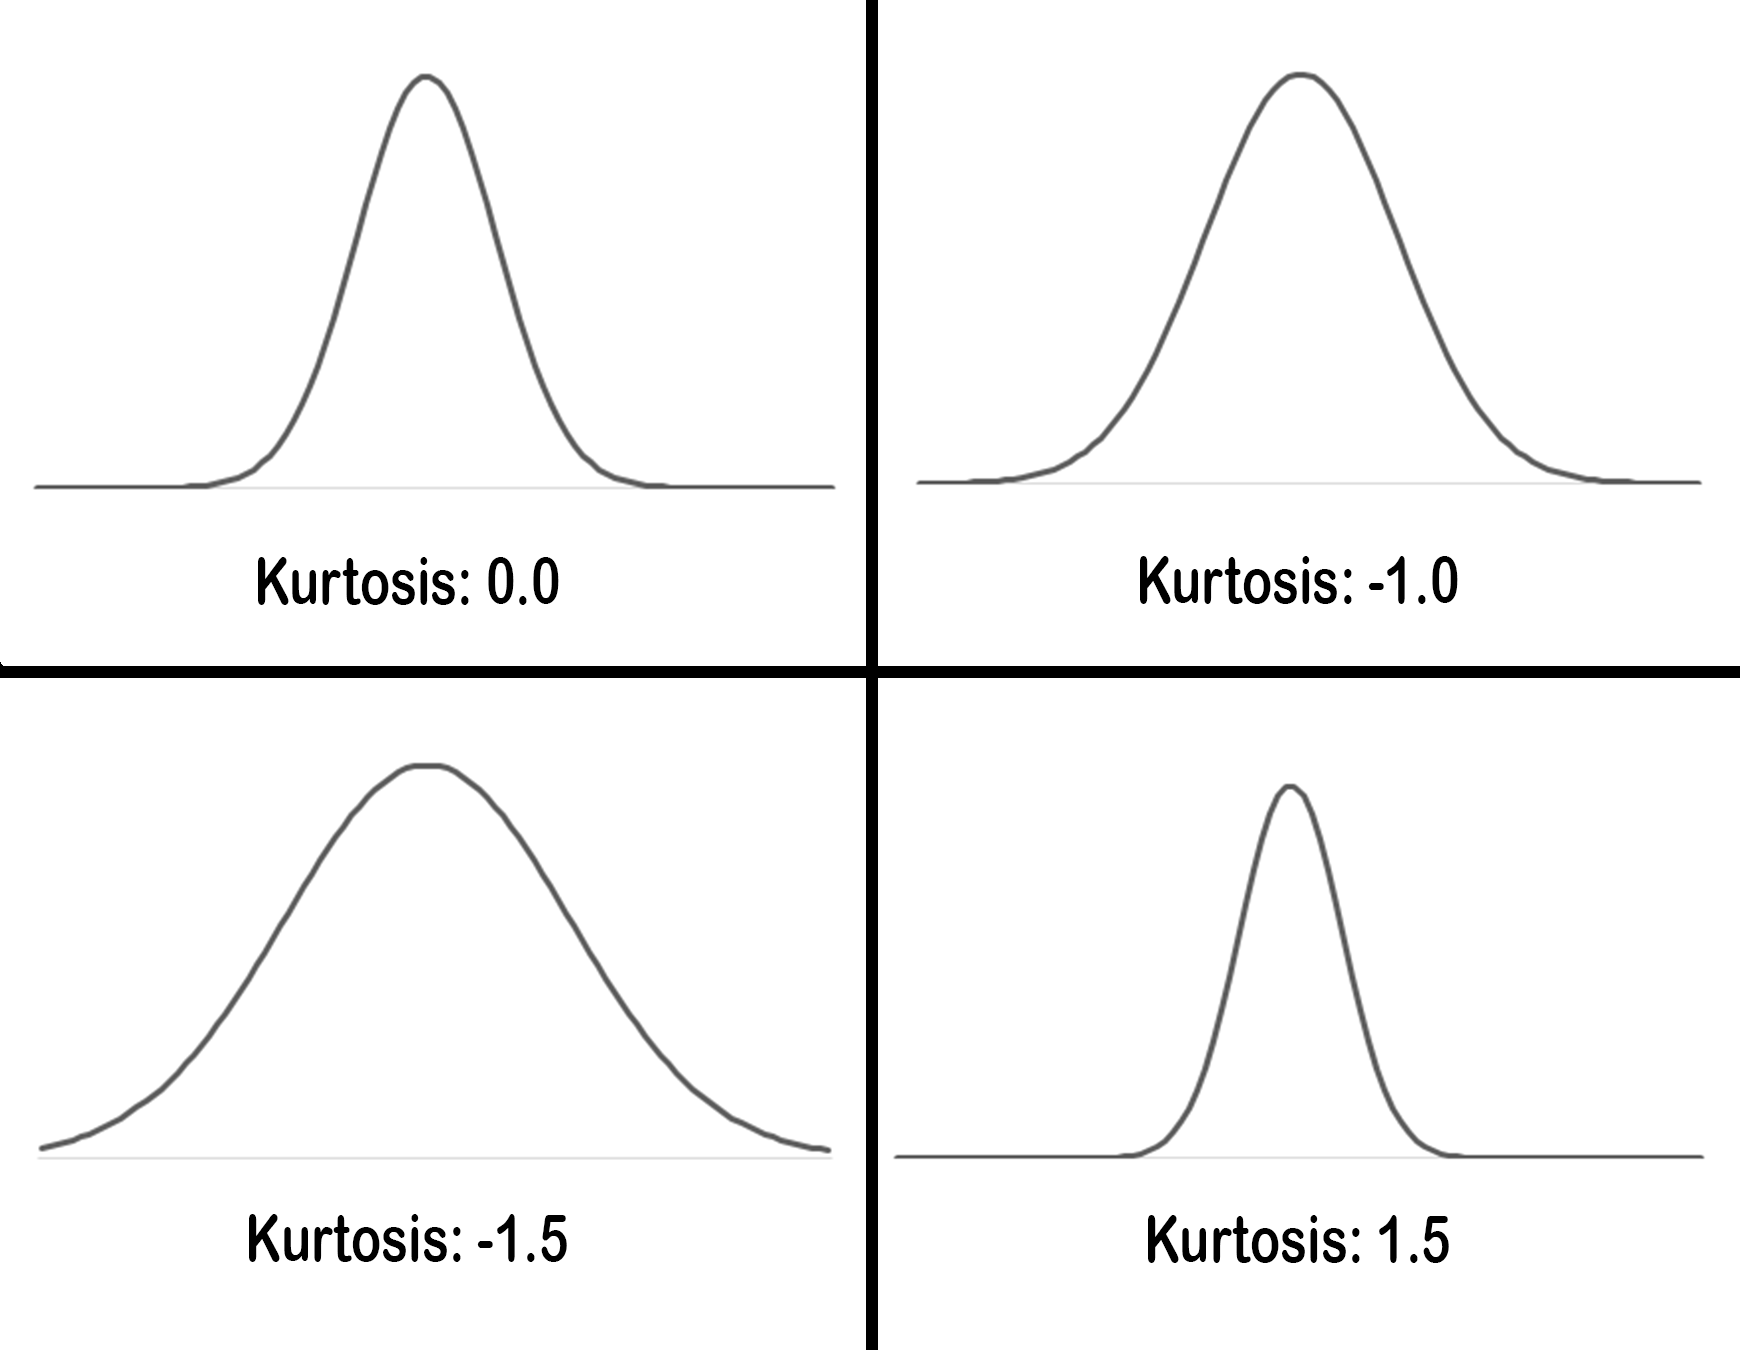
\includegraphics[width=\maxwidth{.95\linewidth}]{gfx/06-Kurtosis}
	\caption{Kurtosis in a Normal Distribution}
	\label{fig06.02}
\end{figure}

\subsection{Skew}
The second numerical measure of a normal distribution that is frequently reported is its \gls{skew}, which is a measure of the symmetry of the curve about the mean of the data. The normal distribution in Figure \ref{fig06.03} has a skew of $ 0.00 $. A positive skew indicates that the tail on the right side is longer, which means that there are several data points on the far right side of the graph ``pulling'' the tail out that direction. A negative skew indicates that the tail on the left side of the graph is longer. Following are three examples of skew:

\begin{figure}[H]
	\centering
	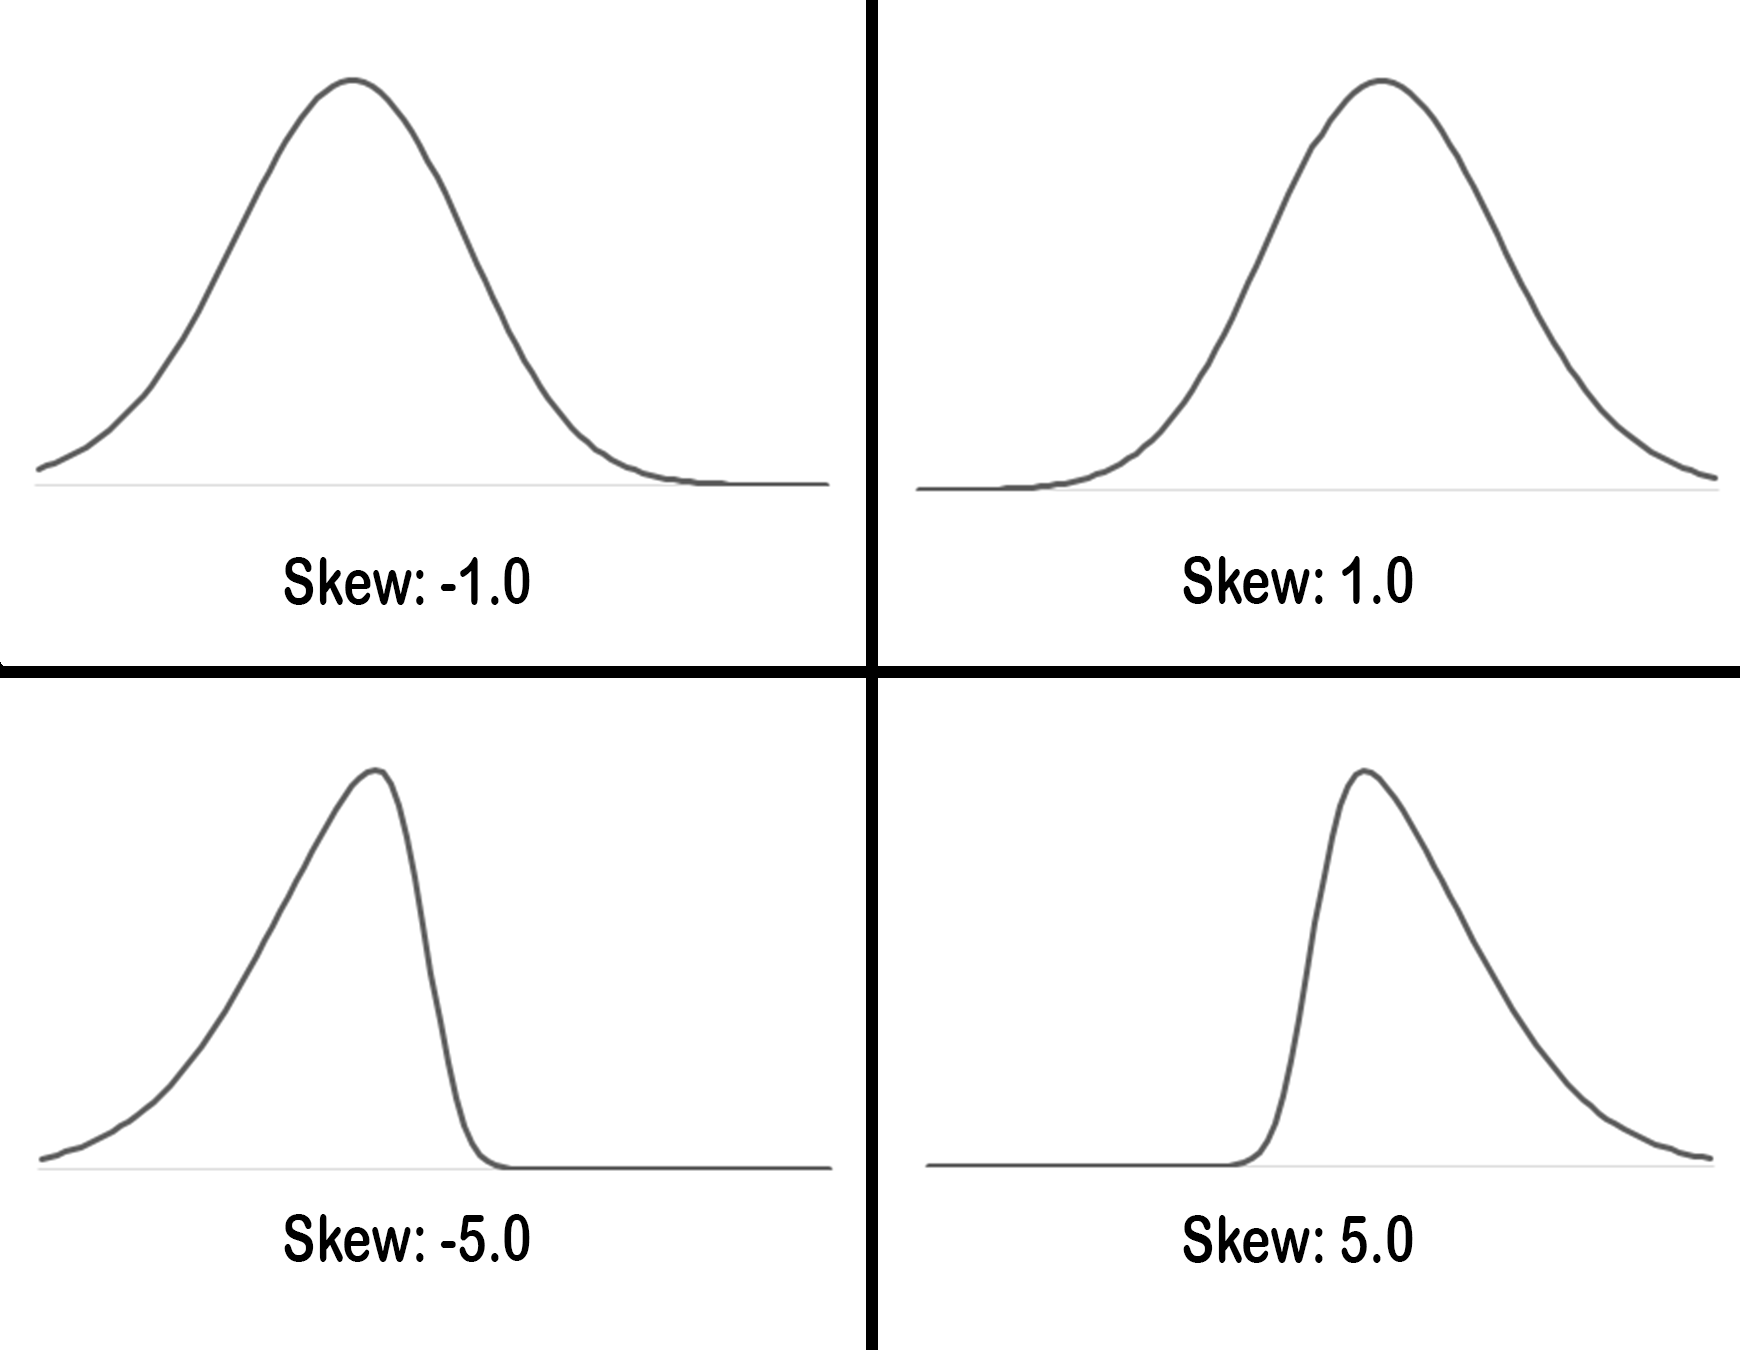
\includegraphics[width=\maxwidth{.95\linewidth}]{gfx/06-Skew}
	\caption{Skew in a Normal Distribution}
	\label{fig06.03}
\end{figure}

\section{Databases}

When a lot of data are gathered into a single location they are referred to as a \gls{database}. This is not a new concept. Fifty years ago a library would have a series of 3X5 cards that contained information about all of the books in the library (title, author, subject, etc.). Those cards were stored in a wooden cabinet called the ``card catalog'' and customers could find information about and the location of whatever book they wanted. Today, databases are often contained in electronic form on the internet where they can be accessed from customers' home computers, tablets, or even phones.

Data in a database is typically stored in tables that resemble spreadsheets, that is, rows and columns where each row is one record (or observation) about some phenomenon and each column is one descriptor of that record. For example, a database that contains information about the people who work at a company would be organized such that each row contained data about just one person and each column would contain a single aspect of that person's employment, like name, employee number, date of birth, etc.\footnote{Of course, databases are much more complex than described in this paragraph but this is not a database text so the simple explanation offered is adequate for this context.} A database is designed to deliver answers to questions through a lookup process so, for example, if the CEO of a company wanted to know the birth date for someone in the accounting department that data could be easily found. 

One common problem with any database is ``dirty data.'' These are data that contain errors or are missing. For example, it is easy for a data entry clerk to enter something like ``1000000'' instead of ``100000'' (count the zeros) for a person's salary and create an ``outlier'' in the data. Another common problem are missing data. For example, if employees are asked to update their personal information but someone could not remember their ZIP code then they would simply leave that field blank.

Dirty data makes it difficult to analyze the database. For example, if a researcher wanted to report the median salary for the workers in a factory but ten percent of the salaries were missing from the database then the median would not be accurate. There are several methods statisticians use to mitigate the problems caused by dirty data but those are beyond the scope of this text. 

\subsection{Public Databases}

There are hundreds of publicly available databases that can be used for research. As one example, the United States Census Bureau maintains a huge database that contains information about the people of the United States.\footnote{The US Census Bureau's website is at \url{https://www.census.gov/}.} The data at that site is freely available to anyone who wants to use it, and the site is organized so information is fairly quick and easy to find. As an example, it is not difficult to discover that among adults in the United States, 29\% have a high school diploma, 20\% have a Bachelor's degree, 8\% have a Master's degree, 1.7\% have a Doctoral degree, and the rest fall elsewhere on the education spectrum. The US Census Bureau has more advanced tools available that permit researchers to focus on a single county or even smaller region.

When using a public database, a researcher must be concerned with bias. Since the researcher did not gather the data first-hand it is possible that the data are biased. For example, if the database includes people's attitude towards work how is the researcher going to know if the data gathered was from a well-designed, neutral survey or if it was just gathered using some sort of convenience sample? In general, databases found at governmental websites (with urls that end with .gov) or education websites (with urls that end with .edu) would more likely be bias-free while databases from .com sites would need to have extra attention paid to bias.

Sometimes, students will find a website with a list of links to journal articles or chapters from books. While these are valuable resources for a researcher, they are not the same as a database that contains raw data from a survey, experiment, or other activity. Journal articles provide good information for a literature review but would not be appropriate for an online database source.

\subsection{Using Public Databases}

As an example of using a public database, imagine that the CEO of ``BASVFOODS'' is interested in opening a neighborhood market in a small town they have never serviced before. In order to gather information about that location it is possible to use US Census Bureau data to find out things like the median household size, income, and education level. The CEO could then compare that data with similar data from a town that has a successful store to help inform a decision to open a new store.

\section{Statistical Analysis}

Once the data are gathered it is important to run some statistical processes to see if the data contains anything of interest. While there are hundreds of tests that can be used, here is a bit of information about the most common tests.

When researchers are determining what type of statistical test to use they must consider the goal of the analysis and the type of data being analyzed. Following are several tables to help determine an appropriate statistical test.

\paragraph{Summary Statistics}

One of the easiest type of analysis to complete is determining the center and spread of a data set. This analysis is also one of the first that research readers expect to find. Here is a guide for what sort of summary test to choose.

\begin{figure}[H]
	\centering

%	\begin{tikzpicture} [outer sep=auto]
%		\node [draw]{Variable}
%			[edge from parent fork down]
%			child {node [draw] {Scale}
%				child {node [draw] {Continuous}}
%				child {node [draw] {Discrete}}
%			}
%			child {node [draw] {Categorical}
%				child {node [draw] {Ordinal}}
%				child {node [draw] {Nominal}}
%			}
%		;
%	\end{tikzpicture}
	\forestset{qtree/.style={for tree={parent anchor=south, 
			child anchor=north,
			align=center,
			inner sep=3pt,
			draw}}}
		
	\begin{forest}, baseline, qtree
		[Variable, fill=purple!40!white
			[{Scale\\(Measure or count)}, fill=cyan!40!white
				[{Continuous\\(Any value)}, fill=cyan!20!white]
				[{Discrete\\(Integers)}, fill=cyan!20!white]
			]
			[{Categorical\\(Tick boxes)}, fill=pink!60!white
				[{Ordinal\\(Ordered)}, fill=pink!40!white]
				[{Nominal\\(No order)}, fill=pink!40!white]
			]
		]
	\end{forest}

	\caption{Classifying Variables}
	\label{fig06.10}
\end{figure}











\begin{table}[H]
	\centering
	\definecolor{ltgray}{gray}{0.95}
	\rowcolors{1}{}{ltgray}
	\begin{tabularx}{0.95\linewidth}{p{0.20\linewidth}p{0.70\linewidth}}
		\toprule
		\textbf{Test} & \textbf{Notes} \\
		\midrule
		{} & \textbf{Association between variables} \\
		Pearson & Correlation between two interval or ratio variables. \\
		Spearman & Correlation between two ordinal variables. \\
		Chi-square & Strength of association between two nominal variables. \\
		\midrule
		{} & \textbf{Difference between means of two variables} \\
		T-test & Difference between two variables. \\
		ANOVA & Difference between two means after other variances are accounted for. \\
		\midrule
		{} & \textbf{Predict one variable from change in another.} \\
		Simple \newline regression & Use a single predictor variable to predict change in another variable. \\
		Multiple regression & Use a multiple predictor variables to predict change in another variable. \\
		\midrule
		{} & \textbf{Tests for qualitative data} \\
		Mann-Whitney & Difference between two categorical variables. \\
		Kruskal-Wallis & Difference between three or more categorical variables. \\
		\bottomrule
	\end{tabularx}
	\caption{My great table.}
	\label{tab06.06}
\end{table}


\subsection{Central Measures}

\subsection{Dispersion}

\subsection{Frequency Tables}

\subsection{Correlation}

\subsection{Parametric Hypothesis Tests}

\subsection{Nonparametric Hypothesis Tests}

\subsection{Data Mining}

\subsubsection{K-Means Clusters}

\subsubsection{Decision Tree}

\begin{figure}[H]
	\centering
	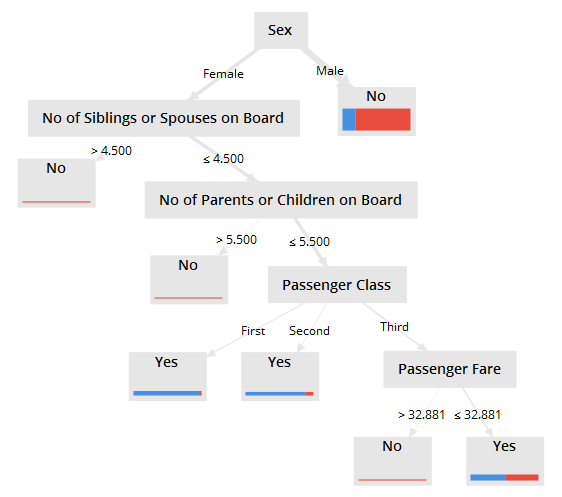
\includegraphics[width=\maxwidth{.95\linewidth}]{gfx/06-DecisionTree}
	\caption{Decision Tree}
	\label{fig06.05}
\end{figure}




\subsubsection{Market Basket}

\begin{figure}[H]
	\centering
	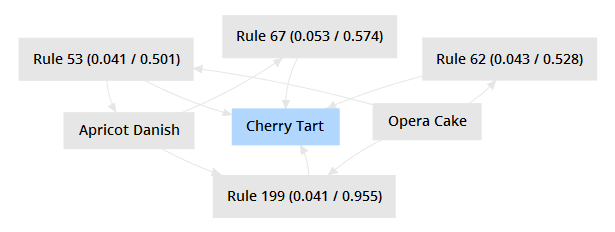
\includegraphics[width=\maxwidth{.95\linewidth}]{gfx/06-MarketBasketGraph}
	\caption{Market Basket Graph}
	\label{fig06.06}
\end{figure}


\begin{figure}[H]
	\centering
	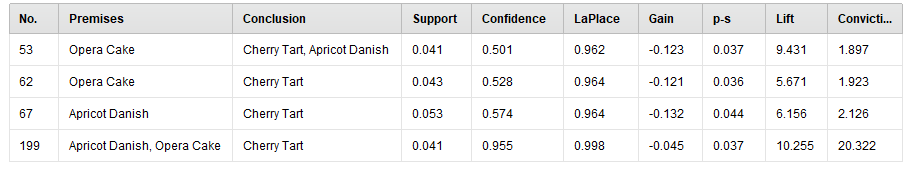
\includegraphics[width=\maxwidth{.95\linewidth}]{gfx/06-MarketBasketRules}
	\caption{Market Basket Rules}
	\label{fig06.07}
\end{figure}


\section{Summary}\label{ch06:summary}

Figure \ref{fig06.04} illustrates the relationship between the various types of data and the rating scales commonly used to work with those data types. Researchers with a positivism philosophy tend to use parametric statistical analysis and gather interval and ratio data. Researchers with an interpretivism philosophy tend to use nonparametric statistical analysis and gather nominal and ordinal data. Nominal data are typically gathered with binary and semantic difference rating scales while ordinal data are typically gathered with Likert and Guttman rating scales.

\begin{figure}[H]
	\centering
	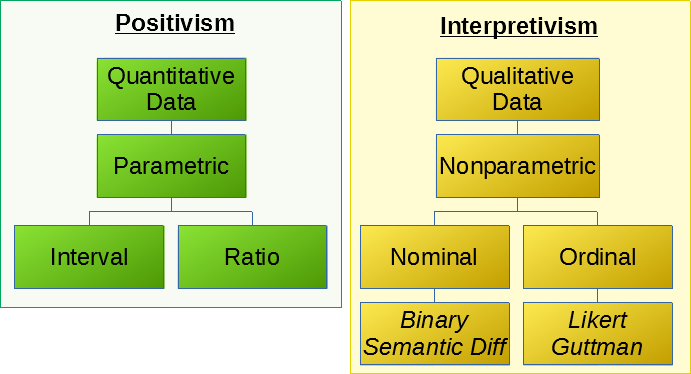
\includegraphics[width=\maxwidth{.95\linewidth}]{gfx/06-DataTypes}
	\caption{Data types}
	\label{fig06.04}
\end{figure}
